\documentclass[10pt,a4paper]{ctexart}
\usepackage[margin=1.8cm]{geometry}
\usepackage{titlesec}
\titlespacing*{\section}{0pt}{1.2ex}{0.7ex}
\usepackage{booktabs,tabularx,array,tikz,graphicx,xurl,hyperref,xcolor}
\graphicspath{{./}{output/pdf/}}
\usetikzlibrary{arrows.meta,positioning}
\hypersetup{colorlinks=true,urlcolor=blue!50!black}
\setlength{\parindent}{2em}
\setlength{\parskip}{0.25em}
\title{AES-128 迭代式加密核设计报告}
\author{李建昊}
\date{2026年9月19日}
\begin{document}
\maketitle
\vspace{-1.5em}
\begin{abstract}
本设计面向低面积、可验证的 AES-128 单块加密。核心使用一块共享同步 S-box ROM，逐字节执行非线性变换，按轮更新密钥。本文给出功能、周期指标、现有综合及物理设计结果、硅后测试方案，并如实列出尚未闭合的 ROM 物理集成问题。
\end{abstract}
\section{功能概述}
核心遵循 AES-128 加密流程，输入 128 位密钥和 128 位明文，输出 128 位密文；包含初始 AddRoundKey、9 轮完整变换，以及省略 MixColumns 的末轮，不支持解密和其他密钥长度。状态采用列优先字节布局。控制器协调状态通路、在线密钥扩展和共享的 $256\times8$ bit 同步 S-box ROM；每轮进行 4 次密钥查询、16 次状态查询，并复用单列 MixColumns 逻辑。外层 \texttt{Aes128Iterative} 将 128 位输入输出映射到 32 位双向数据总线，提供 \texttt{busy}/\texttt{done} 握手，适配 MPC-Frame 的 66 位用户接口。

\begin{figure}[ht]
\centering
\begin{tikzpicture}[>=Latex, node distance=8mm and 12mm, every node/.style={font=\small}, box/.style={draw=blue!60!black,rounded corners=2pt,fill=blue!5,minimum width=30mm,minimum height=10mm,align=center}]
\node[box] (io) {32位 IO 封装\\明文/密钥写入、密文读出};
\node[box,below=of io] (ctrl) {控制器\\轮数与字节计数};
\node[box,below left=11mm and 15mm of ctrl] (key) {当前轮密钥寄存器\\在线密钥扩展};
\node[box,below right=11mm and 15mm of ctrl] (state) {状态寄存器\\ShiftRows / MixColumns / XOR};
\node[box,below=18mm of ctrl,fill=orange!10,draw=orange!70!black] (rom) {共享同步 S-box ROM\\$256\times8$ bit，1个实例};
\draw[->] (io)--(ctrl); \draw[->] (ctrl)--(key); \draw[->] (ctrl)--(state);
\draw[<->] (key)--(rom); \draw[<->] (state)--(rom);
\draw[->] (state.east) -- ++(10mm,0) |- (io.east);
\end{tikzpicture}
\caption{迭代式核心结构示意；ROM 在密钥扩展与状态变换之间分时共享。}
\end{figure}
\section{设计指标}
\begin{center}\small
\begin{tabularx}{\linewidth}{>{\raggedright\arraybackslash}p{35mm}X}
\toprule 指标 & 当前设计与口径 \\ \midrule
功能与接口 & AES-128 单块加密；128 位密钥与数据；32 位分时 IO；同步高有效复位。\\
完成延迟 & 从接受 \texttt{start} 到 \texttt{done} 为 456 个时钟周期；20 MHz 时核心计算约 22.8\,$\mu$s，另加 32 位 IO 装载和读出时间。\\
吞吐率 & 连续单块核心计算上限约 $20\,\mathrm{MHz}/456\times128=5.61$ Mbit/s；实际系统吞吐率还受 IO 协议和帧控制影响。\\
设计侧重点 & 面积优先，采用单 ROM 与运算复用；性能和功耗为次要目标。\\
验证状态 & RTL 单元、核心和 IO 封装测试可运行；现有物理结果仍需完成 ROM 宏集成复核。\\
\bottomrule
\end{tabularx}
\end{center}
\section{综合与 ECOS Studio 物理结果}
现有 ECOS 后端运行以 \texttt{Aes128Iterative} 为顶层。其 Yosys 综合报告列出 \textbf{3620 个实例}，其中 1 个为面积未知的 ROM 宏实例；\textbf{3619 个标准单元}面积为 \textbf{9751\,$\mu$m$^2$}。ROM 的典型 Liberty 文件给出 1761.372\,$\mu$m$^2$，二者相加约 11512.4\,$\mu$m$^2$，仅作为未加布线、填充与物理开销的粗略估算。

\begin{center}\small
\begin{tabularx}{\linewidth}{>{\raggedright\arraybackslash}p{40mm}X}
\toprule 项目 & ECOS Studio 后端 Key Metrics（四舍五入） \\ \midrule
版图面积与利用率 & Die 34003\,$\mu$m$^2$；core 利用率 30.0\%（数据库精度 30.28\%）；die 利用率 28.98\%。\\
标准单元与实例 & 3650 个标准单元，面积 9855\,$\mu$m$^2$（数据库精度 9854.6）；总实例数 12609，含填充等物理单元，不能视为逻辑门数。\\
宏与接口 & Macro Number 0，Macro Area 0\,$\mu$m$^2$；IO Pin 200，IO Pad 0；net 3822。\\
时序摘要 & 页面显示 Frequency 347 MHz；setup WNS $+0.448$ ns、TNS 0 ns；hold WNS $+0.087$ ns、TNS 0 ns。频率为该次工具报告值，不等于硅片保证工作频率。\\
物理检查 & 现有 iLVS 摘要报告 0 open、0 short；检查范围仍缺少实际放置的 ROM 宏。\\
\bottomrule
\end{tabularx}
\end{center}
\begin{figure}[ht]
\centering
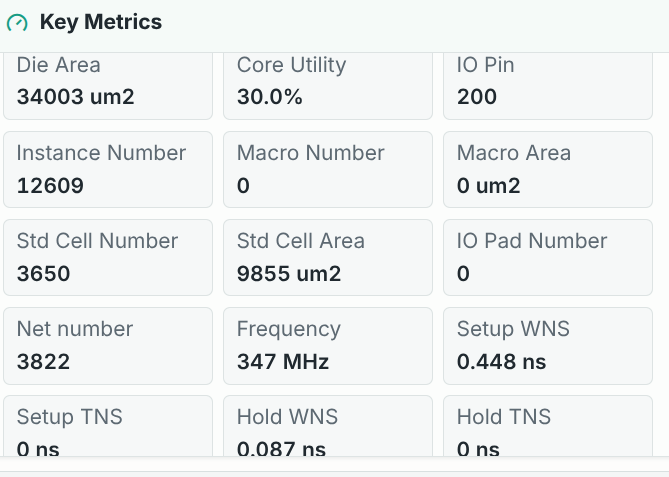
\includegraphics[width=0.82\linewidth]{key_metrics.png}
\caption{ECOS Studio 后端 Key Metrics 原始截图。}
\end{figure}
以上 3650/9855 为后端阶段数据；前述 3619/9751 为综合阶段数据，两者阶段及统计口径不同。后端总实例数 12609 随填充单元加入而增加，不应与综合单元数直接比较。
\noindent\textbf{流片前关键限制：}后端日志出现 \texttt{can not find cell master = ics55\_ecos\_rom\_256x8\_m8\_b1}，后端 Key Metrics 中 Macro Number 与 Macro Area 均为 0。因此上述 ECOS die/core 面积、利用率、时序及物理检查\textbf{未包含正确放置的 ROM 宏}，不能作为完整芯片的最终面积或签核结果。须导入并核对 ROM LEF/GDS/Liberty、内容映射和电源连接，重新完成布局布线、时序、DRC 与 LVS，再更新正式指标。

\section{回片后测试方法及预期效果}
回片交付的是单颗芯片，需先依据最终封装与引脚定义设计专用测试 PCB，布置电源、去耦、复位、时钟及 FPGA 接口连接，并预留必要的测量点。芯片焊接到 PCB 后，先检查焊点、供电电压、短路及各接口连通性，再连接 FPGA 进行功能测试。PCB 设计与制板、芯片焊接及板级联调是硅后验证的必要环节；具体焊接工艺应以实际交付的芯片封装形式为准。

使用 FPGA 与测试板提供同一测试时钟。上电后保持同步复位至少 20 个上升沿；先以 100 kHz 或 1 MHz 验证接口，再逐级提高频率。FPGA 在下降沿设置 32 位数据、字序与控制信号，ASIC 在上升沿采样；按 4 个字分别写入密钥和明文，发送单周期 \texttt{start}，监测 \texttt{busy} 与单周期 \texttt{done}，超时门限设为大于 456 周期。读密文前 FPGA 释放双向总线，依次读取 4 个字并重组 128 位结果。

首要已知答案测试采用 FIPS-197 示例：\par\noindent\texttt{Key = 000102030405060708090a0b0c0d0e0f}\par\noindent\texttt{PT  = 00112233445566778899aabbccddeeff}\par\noindent\texttt{CT  = 69c4e0d86a7b0430d8cdb78070b4c55a}。随后运行全零、递增、随机向量，并与软件参考模型逐块比对；重复启动及复位中断测试检查状态清除和握手行为。预期所有密文完全一致、无总线争用，且 \texttt{done} 相对启动为 456 周期；再记录不同频率与电压下的通过率和供电电流。频率与功耗的最终值应以硅片实测为准。

\section{其他说明}
项目采用 Verilog-2005 加密核心，ROM 仿真模型与物理宏须分别管理。面积优化通过共享 S-box、在线密钥扩展及按列复用 MixColumns 实现；代价是较长的单块延迟。开源仓库：\par\noindent\url{https://github.com/Briarcresy/AES-128-Core-Iterative}。\par 本报告数据依据本地 \texttt{docs/architecture.md}、\texttt{docs/interface.md}、\texttt{backend/workspace/Synthesis\_yosys} 、\texttt{backend/workspace/route\_ecc} 与 \texttt{backend/workspace/sta\_ecc} 报告；面积与利用率属于当前工程快照，并非最终流片签核承诺。
\clearpage
\thispagestyle{plain}
\begin{figure}[ht]
\centering
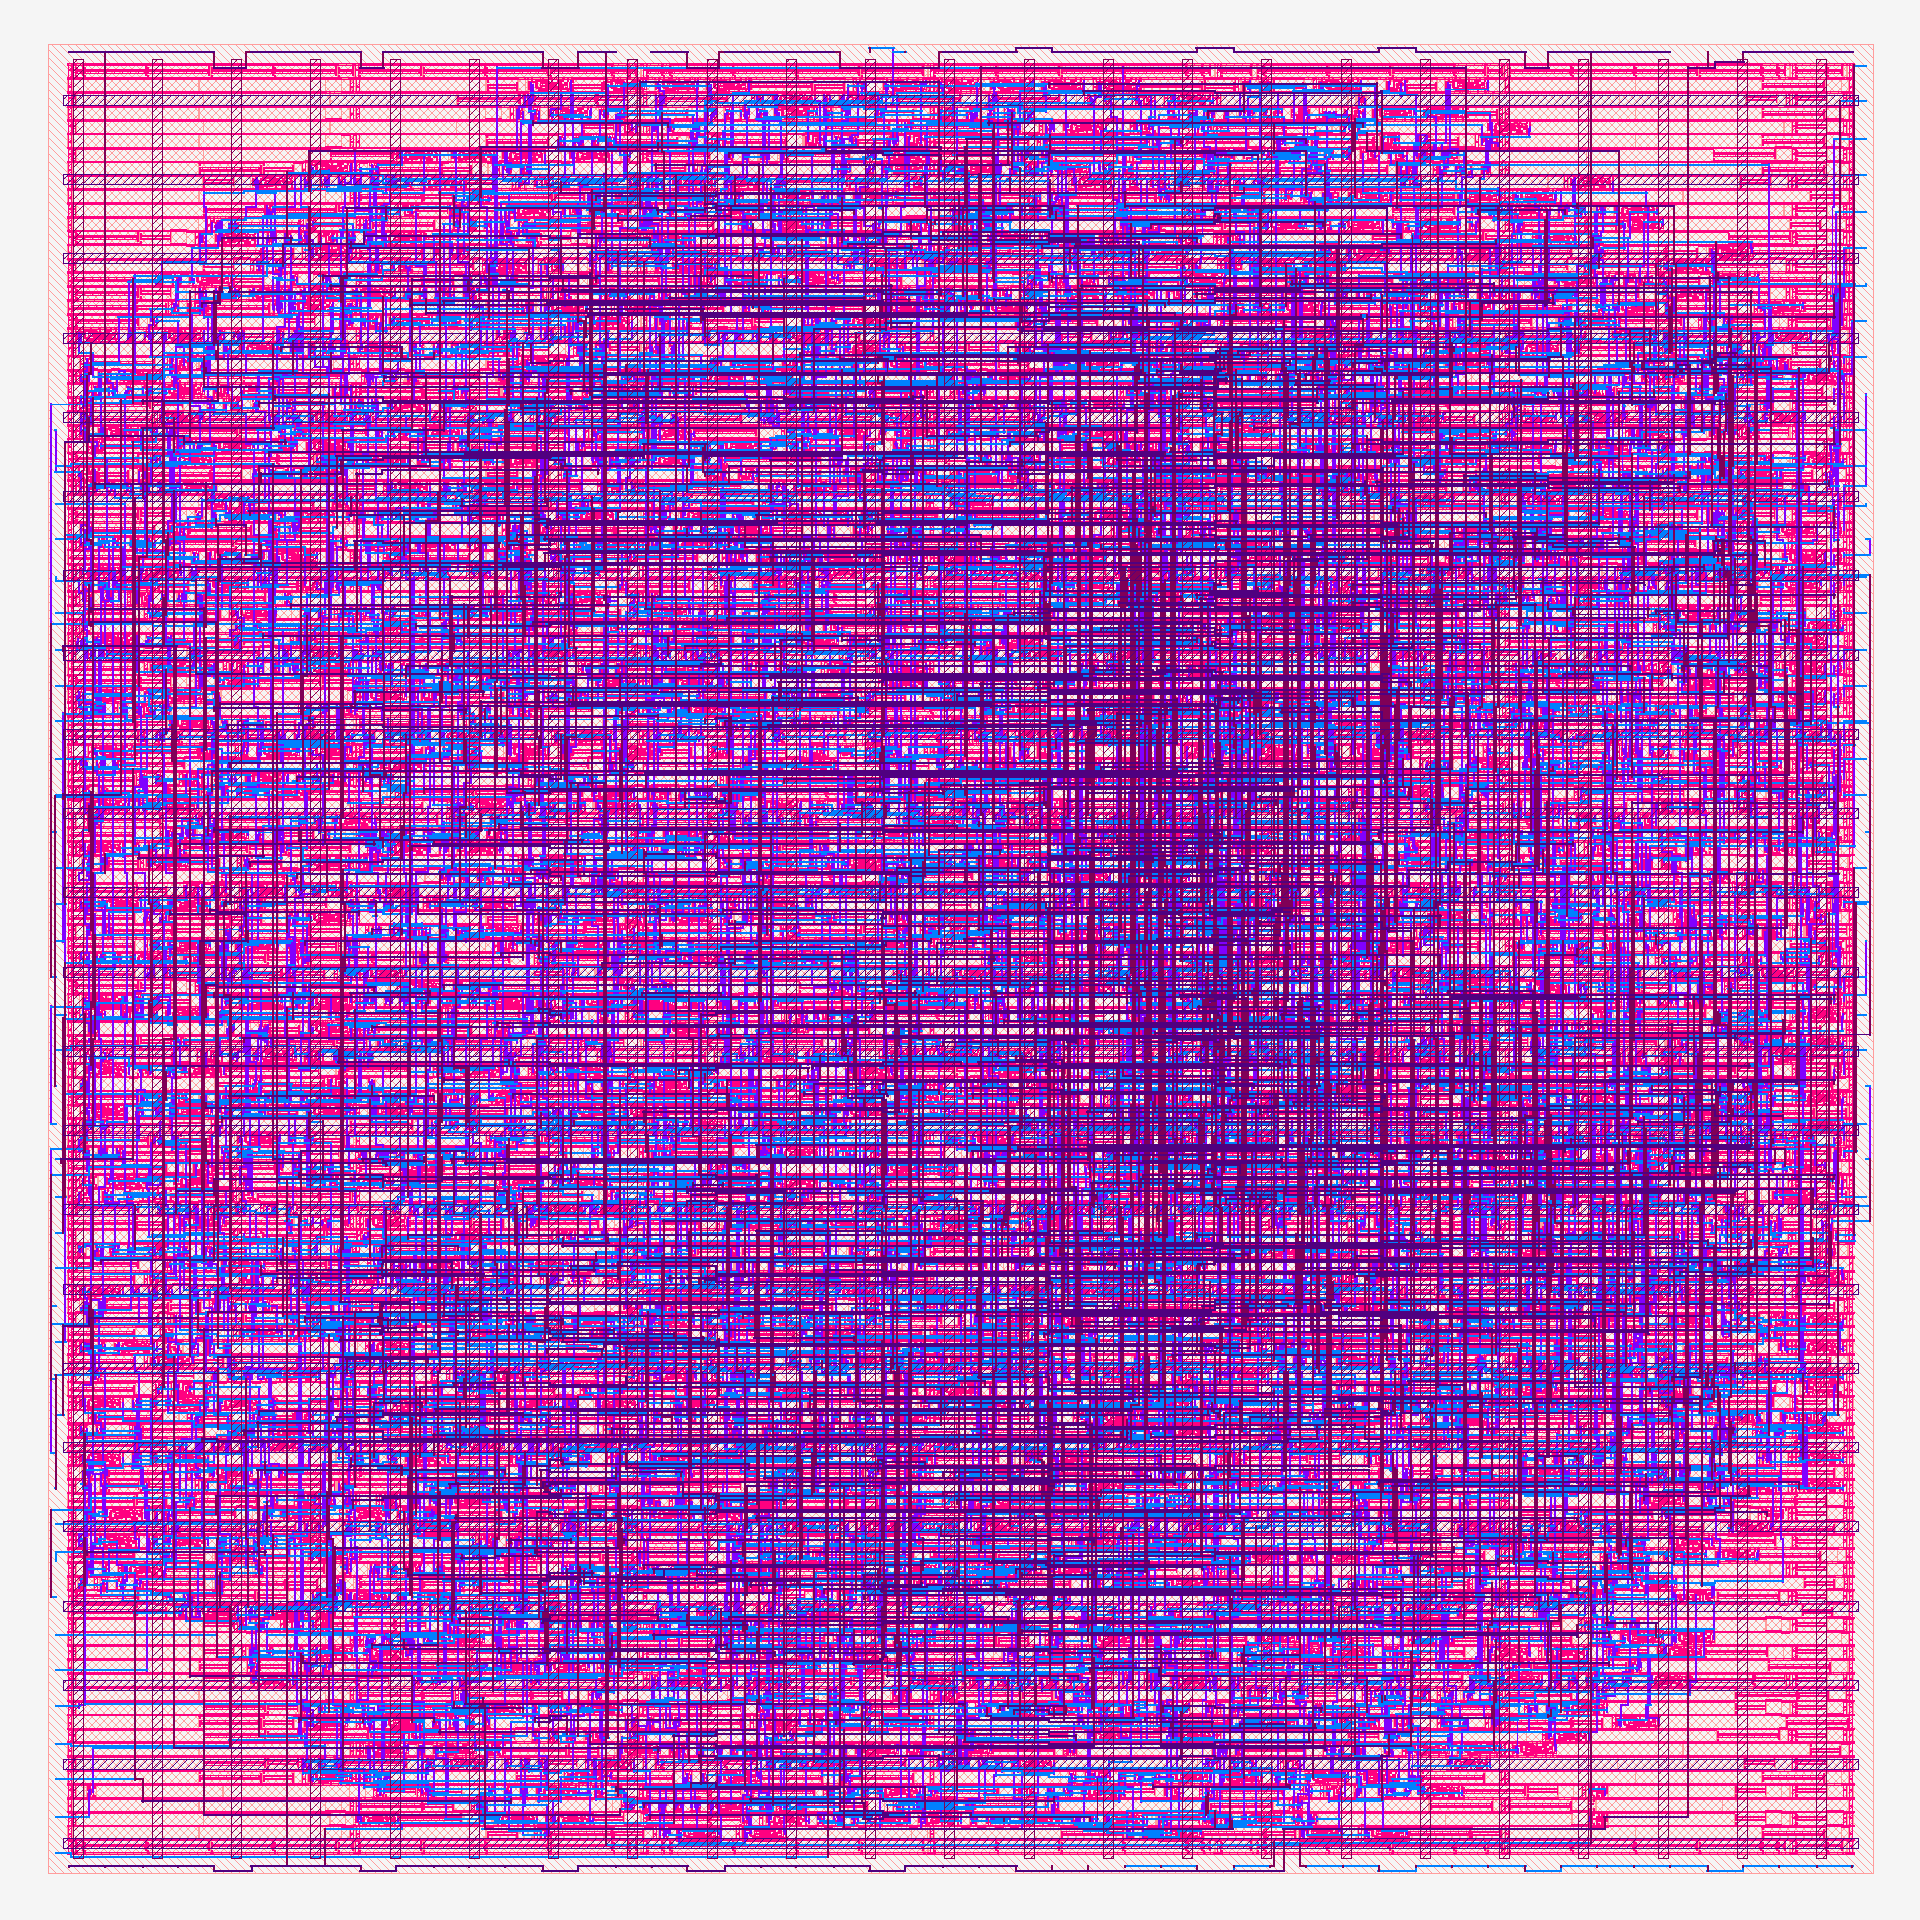
\includegraphics[width=0.78\linewidth,height=0.72\textheight,keepaspectratio]{aes128-iterative.png}
\caption{ECOS Studio 后端生成的 AES-128 设计版图图像（final/design）；该工程快照尚未正确集成 S-box ROM 宏。}
\end{figure}
\end{document}
